\section{Methodology of \tool}

\begin{figure*}[ht]
    \centering
      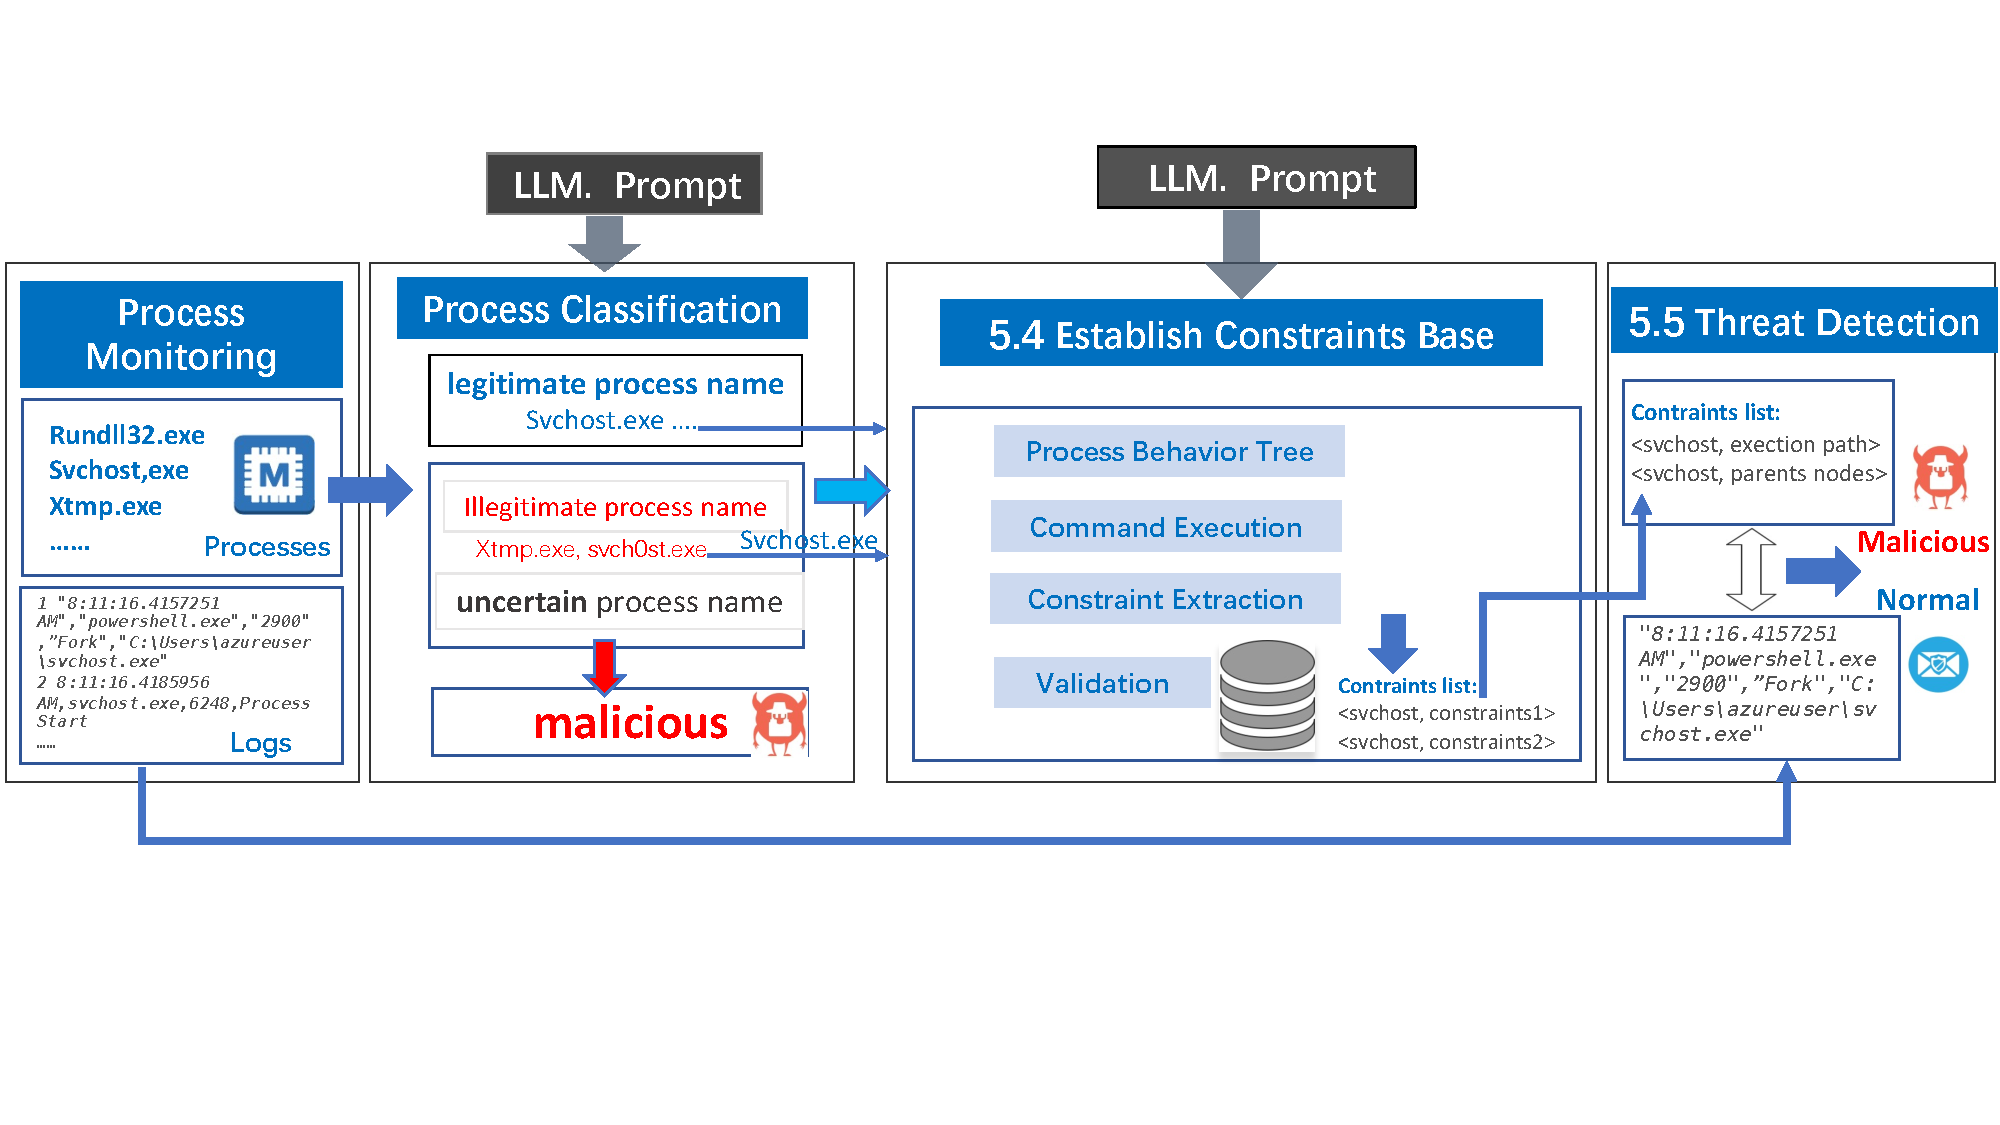
\includegraphics[width=0.95\textwidth]{figs/framework.pdf}
    \caption{The system process logs are collected and categorized using LLM as legitimate, illegitimate, and uncertain processes. Processes labeled uncertain or illegitimate are flagged for security analyst review (detailed in Section~\ref{sec:classifition}). If determined to be legitimate, LLM assists in the creation of a database of process constraints. This is achieved through behavior tree creation, command execution, constraint extraction and validation (explained in Section~\ref{sec:profile_con}). Logs that violate these constraints are indicative of potential threats (detailed in Section~\ref{sec:Threat_detection}).}
    \label{fig-framework}
    \end{figure*}

\subsection{Threat Model}
We will begin by defining a threat model in this paper. This project aims to address the threat of APT attacks targeting critical entities that have been identified as critical infrastructure. These attacks have the following characteristics:

\begin{itemize}
    \item \textbf{Stealthy}. Instead of simply performing an attack, the attacker consciously hides their malicious activities, trying to mix their behavior with a large amount of benign background data, which makes the victim system perform like a benign mode.
    \item \textbf{Evolving}. As professional attacker groups continue to innovate, they are targeting an ever-expanding range of system processes and adapting to the latest defensive measures in order to stay ahead of the game. 
    \item \textbf{Frequent usage of zero-day exploits}. The attacker tends to use zero-day exploits to attack a system. Therefore, we assume that there are no attack patterns for training.
\end{itemize}
As an alternative to sample-focused analysis, we propose to observe ubiquitous OS kernel processes. The system processes are always present and do not need to be identified before analysis, unlike suspicious samples.

\subsection{Technical Challenges}

How can we efficiently extract these constraints? It's a crucial question. Fortunately, LLMs offers significant advantages when it comes to building process profiles due to its exceptional knowledge extraction capabilities.
However, we found that using LLMs construction processes directly posed the following three technical challenges.

% \circled{1} Complexity Handling: It might be difficult for LLMs to give comprehensive solutions when they are faced with complicated questions or scenarios.

\noindent
{\bf CH-\circled{1} Context Dependency.} %  : 
In order to provide accurate results, LLMs often require a rich contextual environment. In the absence of this, their responses can be generic or imprecise. 

\noindent
{\bf CH-\circled{2} Memory Limitations.} % \circled{2}
Due to its token limit, LLMs cannot handle excessively long texts. In addition, LLMs tend to focus more on recent interactions and overlook previous details in a conversation history. 

\noindent
{\bf CH-\circled{3} Hallucinations.} % \circled{3} 
This is a risk that might reveal plausible-looking yet factually unsupported or nonexistent information if the model does produce hallucinations. 

% Therefore, the key to building process profiles using LLMs is overcoming these challenges which is the central focus of this paper.

\subsection{Overview of \tool}
As illustrated in Figure~\ref{fig-framework}, we accessed a log collection tool to collect logs from a variety of system processes that were running at different times in the system. Utilizing the powerful capabilities of LLMs, we were able to categorize these processes based on their names into three distinct categories: legitimate process names, illegitimate process names, and uncertain process names (due to the inherent incompleteness of the GPT's database). As for the latter two categories, we classified them as potentially malicious, requiring more investigation by security analysts in order to determine whether they are malicious or not. A more in-depth examination of this process is provided in Section~\ref{sec:classifition}.

As for processes that were classified with legitimate names, we used the LLMs to construct a database that outlined the normal constraints of the process.

In a previous Section~\ref{sec:intuition}, we briefly discussed the four challenges that exist when building process profiles based on the LLMs model. To address these challenges, we developed ProfileGuard, a method that harnesses LLMs for the automated creation of critical system process profiles based on the information provided by LLMs. ProfileGuard acts as a security guard for the system, using system process profiles to prevent malicious attackers.
We broke down the comprehensive profiling task into four manageable subtasks:
\begin{itemize}
    \item \textbf{Process Behavior Tree Construction}: Our goal was to capture a comprehensive range of behaviors for each process, creating a behavior tree. Through a "self-ask" approach, the LLMs continuously expanded its knowledge of this tree. LLMs can benefit greatly from this tree as it provides context for {\bf CH-\circled{1}}.
    \item \textbf{Command Execution}: A behavior tree was used to guide the LLMs to script and execute commands for behaviors that could be addressed. In addition, command execution generates richer contextual information for {\bf CH-\circled{1}}, and checks simple constraints, such as execution paths and parent-child relationships.
    \item \textbf{Constraint Extraction}:  In this step, we'll combine the LLMs and traditional programs to solve {\bf CH-\circled{2}}. Since the log size is large, asking GPT directly will easily exceed its memory limit and cause previous information to be lost. We employed common term and prefix-span sequence mining to discover deeper relationships between logs. Each constraint, which was identified by LLMs, was interpreted using its knowledge.
    \item \textbf{Validation}: LLMs must be accurate and consistent due to potential hallucination issues. We've implemented a two-tier validation approach to validate the model's outputs for {\bf CH-\circled{3}}. The first tier involves executing actual commands and cross-checking with real-world logs. Multiple LLMs engage in a multi-round debate to mutually verify their respective responses and reasoning, aiming to arrive at a unified conclusion.
\end{itemize}

Leveraging this process behavior database, we compared extracted log information against the established constraints. Any violation of these constraints is indicative of potential malicious activity.
A detailed discussion on this topic is set out in Section~\ref{sec:Threat_detection}. 






